\setcounter{chapter}{3}
\chapter{Il Moto del Corpo Rigido}
\section{Introduzione}
\begin{wrapfigure}{r}{0.3\textwidth}
\vspace{-0.4in}
  \begin{center}
    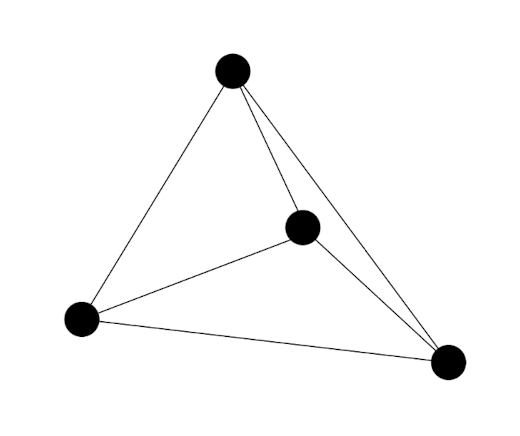
\includegraphics[width=0.35\textwidth]{rigid}
  \end{center}
\end{wrapfigure}
In questa trattazione consideriamo corpi estesi che non possiedo gradi di libert\`{a} internamente alla loro struttura. Corpi di questo tipo prendono il nome di \textbf{corpi rigidi}, e li modellizziamo considerandoli come una collezione di N punti materiali vincolati tra loro rigidamente. Ovvero la distanza tra di essi \`{e} costante.
\begin{equation}
	|\bm{r}_{i} - \bm{r}_j| = \text{costante} \quad \forall \; i,j = 1,..,N
\end{equation}
Un corpo rigido nello spazio \`{e} descritto da sei gradi di libert\`{a}
\begin{center}
	3 Traslazione + 3 Rotazione
\end{center}
Il moto pi\`{u} comune che pu\`{o} assumere \`{e} dato da una roto-traslazione dei suoi punti. Nelle sezione successive svilupperemo gli strumenti necessari a descrivere questo tipo di moto utilizzando gli strumenti della meccanica Lagrangiana.

\section{Cinematica}
\subsection{Olonomia del vincolo di rigidit\`{a}}
Innanzitutto verifichiamo che un corpo rigido possa essere descritto con gli strumenti della meccanica Lagrangiana, ovvero verifichiamo che i vincoli di rigidit\`{a} sui punti, e dunque le forze interne presenti nel sistema, rappresentino una condizione di vincolo liscio.
\newline
Abbiamo che 
\begin{equation}
	\frac{d}{dt}||\bm{r}_i(t) - \bm{r}_j(t)||= \langle \dot{\bm{r}}_i - \bm{\dot{r}}_j,\bm{r}_i - \bm{r}_j\rangle  = 0
\end{equation}
dunque le velocit\`{a} relative sono ortogonali  alla direzione congiungete tra le posizioni dei punti materiali per ogni tempo. La potenza del vincolo complessiva \`{e} data da 
\begin{equation}
	\pi_{tot} = \bm{R} \cdot \bm{\dot{v}} = \bm{\phi}_j \cdot  \bm{\dot{r}}_j + \bm{\phi}_i \cdot \bm{\dot{r}}_i
\end{equation}
la relazione vincolare $\bm{{\phi}}_j$ rappresenta la forza esercitata dal punto j sul punto i, e quindi \`{e} diretta lungo la congiungente dei due punti. Analogamente vale il viceversa per $\bm{\phi}_i$. Entrambe hanno stesso modulo ma verso opposto.
\begin{equation}
	\bm{\phi}_j = \alpha(\bm{r}_i - \bm{r}_j) \quad \text{e} \quad \bm{\phi}_i = - \alpha(\bm{r}_i - \bm{r}_j)
\end{equation}
dunque la 4.3 diventa 
\begin{equation}
\begin{aligned}
\pi_{\text {tot }} & =\alpha\left(\bm{r}_i-\bm{r}_j\right) \cdot \dot{\bm{r}}_i-\alpha\left(\bm{r}_i - \bm{r}_j\right) \cdot \dot{\bm{r}}_j= \\
& =\alpha\left(\bm{r}_i-\bm{r}_j\right) \cdot\left(\bm{r}_i-\dot{\bm{r}}_j\right)=0
\end{aligned}
\end{equation}
dunque possiamo concludere che i vincoli di rigidit\`{a} di un corpo rigido sono dei vincoli lisci.

\subsection{Spazio delle configurazioni}
Consideriamo un corpo con un punto fissato P nello spazio e che sia libero di ruotare attorno ad esso. Per descrivere il moto abbiamo bisogno di definire un sistema di riferimento fisso (sistema del laboratorio) la cui base \`{e} data da $\{\bm{\tilde{e}}_a \}$ e un sistema di riferimento mobile sovrapposto e solidale con il corpo descritto da una base $\{\bm{e}_a(t)\}$. Dove rispettivamente gli assi descritti dalle basi sono ortogonali tra loro 
\begin{equation}
\tilde{\mathbf{e}}_a \cdot \tilde{\mathbf{e}}_b=\delta_{a b} \quad, \quad \mathbf{e}_a(t) \cdot \mathbf{e}_b(t)=\delta_{a b}
\end{equation}

\begin{figure}[!ht]
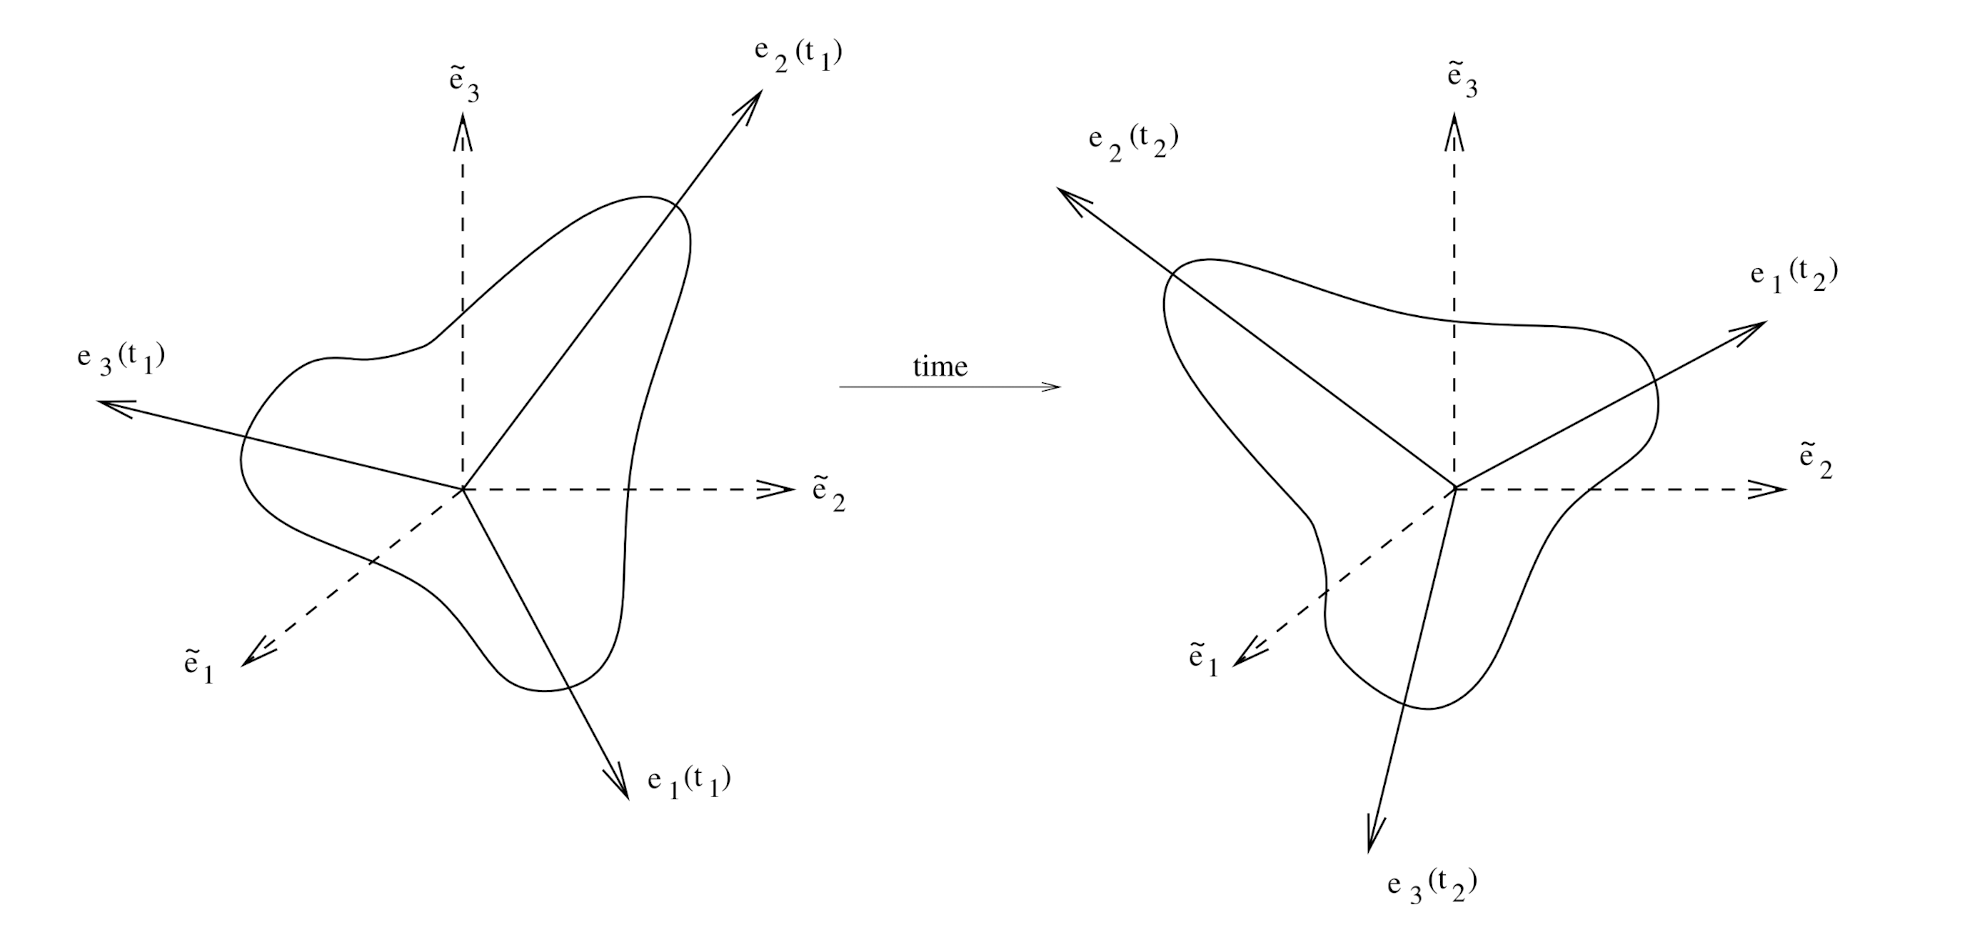
\includegraphics[width= 14cm]{rotation}	
\centering

\end{figure}
Per descrivere le rotazioni nello spazio utilizziamo la matrice $R \in SO(3)$, che gode della propriet\`{a} per cui la sua inversa, coincide con la trasposta, ovvero 
\begin{equation}
R \cdot R^{T} = R^{T} \cdot R = I  \Rightarrow R^{T} = R^{-1}	
\end{equation}
e possiede determinante non nullo, e quindi \`{e} una mappa invertibile. Prendiamo un punto $\bm{x}$ appartenente al corpo rigido, questo pu\`{o} essere espresso rispetto alla base del SR del laboratorio come 
\begin{equation*}
	\bm{\tilde{x}} = \sum_{i}\tilde{x}_i\; \bm{\tilde{e}}_i
\end{equation*}
di conseguenza quando facciamo agire la matrice R sul vettore, questa in realt\`{a} trasforma la base rispetto alla quale espresso 
\begin{equation}
	\bm{x} = R\bm{\tilde{x}} = \sum_{i}\tilde{x}_i\; R\bm{\tilde{e}}_i = \sum_{i}x_i\;\bm{e}_i 
\end{equation}
di conseguenza 
\begin{equation*}
	\bm{e}_i = \sum_{i}  R\bm{\tilde{e}}_i
\end{equation*}
dove le singole componenti sono esprimibili come 
\begin{equation*}
	x_i = \sum_{k}R_{ik}\tilde{x}_{k} \quad e_j^i = \sum_{k} R_{ik} \tilde{e}_k
\end{equation*} 
\subsection{Velocit\`{a} Angolare}
Esprimiamo la velocit\`{a}  rispetto al sistema di Laboratorio come 
\begin{equation}
	\frac{d\bm \tilde{x}}{dt} = \sum_{i} \dot{\tilde{x}}_i \; \tilde{e}_{i}
\end{equation}
mentre rispetto al sistema comovente si ha 
\begin{equation}
	\frac{d\bm{x}}{dt} = \sum_{i} x_{i} \frac{d \bm{e}_i}{dt}
\end{equation}
per la singola componente della derivata $\frac{d \bm{e}_i}{dt}$ si ha che 
\begin{equation}
	\frac{d e_{j}}{dt} = \sum_{k} \frac{d R_{jk}}{dt} \; \tilde{e}_k = \sum_{k} \dot{R}_{jk} \; \tilde{e}_k
\end{equation}
poich\`{e} l'applicazione lineare R \`{e} invertibile si ha che la componente k-sima di un vettore della base del SR del laboratorio \`{e} esprimibile come 
\begin{equation}
	\tilde{e}_k =\sum_{m} R^{-1}_{km} e_m
\end{equation}
di conseguenza la velocit\`{a} rispetto al SR solidale al corpo rigido \`{e} data da 
\begin{equation}
	\dot{\bm{x}}= \sum_{k,m = 1}\underbrace{(R^T\dot{R})_{mk}}_{A} \; \underbrace{\tilde{x}_k \; \bm{e}_m}_{B}
\end{equation}
dove la parte A esprime la dinamica rotazionale che \`{e} indipendente dalla scelta dal punto, mentre la parte B recupera tale informazione. 
Le  matrici R(t) e $\dot{R}(t)$ per una rotazione attorno ad un polo fisso P sono definite come
\begin{equation}
R=\left[\begin{array}{cc}
\cos \theta & -\sin \theta \\
\sin \theta & \cos \theta 
\end{array}\right] \quad \text {e} \quad  \dot{R}=\left[\begin{array}{rr}
-\sin \theta \dot{\theta} & -\cos \theta \dot{\theta} \\
\cos \theta \dot{\theta} & -\sin \theta \dot{\theta}
\end{array}\right]
\end{equation}
di conseguenza il prodotto
\begin{equation}
R^{\top} \dot{R}=\left[\begin{array}{cc}
\cos \theta & \sin \theta \\
-\sin \theta & \cos \theta
\end{array}\right]\left[\begin{array}{cc}
-\sin \theta \dot{\theta} & -\cos \theta \dot{\theta} \\
\cos \theta \dot{\theta} & -\sin \theta \dot{\theta}
\end{array}\right] = 
\left[\begin{array}{cc}
0 & -\dot{\theta} \\
\dot{\theta} & 0
\end{array}\right]
\end{equation}
che \`{e} una matrice anti-simmetrica. La velocit\`{a} rispetto al SR mobile \`{e} data da 
\begin{equation}
	||\bm{\dot{x}}||^2 = \dot{\theta}^2 \left (\tilde{x}_1^2 + \tilde{x}_2^2 \right) =  \dot{\theta}^2 \left (x_1^2 + x_2^2 \right) = \dot{\theta} ||\bm{x}||^2 
\end{equation}
La lunghezza del vettore posizione del punto P \`{e} un invariante rispetto all'azione della matrice di rotazione. Quella che cambia \`{e} la velocit\`{a} con cui viene descritto lo spostamento.
\newline 
Se consideriamo un asse la cui direzione \`{e} ortogonale al piano di rotazione e passante per il punto P, abbiamo che data la velocit\`{a} angolare rispetto ad esso \`{e} data dall'equazione
\begin{equation}
	\bm{\Omega} = \dot{\theta}\,\bm{e}_3
\end{equation}
e si lega all'espressione della velocit\`{a} mediante l'operatore di prodotto vettoriale nel seguente modo
\begin{equation}
\bm{\Omega} \times \bm{x}_p=\operatorname{det}\left[\begin{array}{ccc}
\bm{e}_1 & \bm{e}_2 & \bm{e}_3 \\
0 & 0 & \dot{\theta} \\
\tilde{y}_1 & \tilde{y}_2 & \tilde{y}_3
\end{array}\right]= \bm{e}_1 (-\dot{\theta}\tilde{x}_2) - \bm{e}_{2} (-\dot{\theta}\tilde{x}_1) = \bm{\dot{x}}_{P}
\end{equation}
\subsection{Energia Cinetica}
Utilizzando il punto P appartenente al corpo rigido possiamo esprimerlo rispetto al SR del laboratorio come 
\begin{equation}
	\bm{\dot{\tilde{x}}}_{P} = \bm{\dot{x}}_{O} + \bm{\dot{x}}_{P}
\end{equation}
quindi l'energia cinetica \`{e} esprimibile come 
\begin{equation}
\begin{aligned}
& K=\frac{1}{2} \sum_{p=1}^N m_p\left\|\bm{\dot{\tilde{x}}}_p\right\|^2= \frac{1}{2} \sum_{p=1}^N m_p\left(\dot{\bm{x}}_0+\dot{\bm{x}}_p\right) \cdot\left(\dot{\bm{x}}_0+\dot{\bm{x}}_p\right) = \\[0.2in]
& = \frac{1}{2} \sum_{p=1}^N m_p\left(\left\|\dot{\bm{x}}_0\right\|^2+2\left\langle\dot{\bm{x}}_0, \dot{\bm{x}}_p\right\rangle+\|\dot{\bm{x}}_ p\|^2\right) = \\[0.2in]
& = \frac{1}{2}\left(\sum_{p=1}^N m_p\right)\left\|\bm{\dot{x}}_0\right\|^2+\frac{1}{2} \sum_{p=1}^N m_p\left\|\dot{\bm{x}}_p\right\|^2+\left\langle\bm{\dot{x}}_0, \sum_{p=1}^N m_p \dot{\bm{x}}_p\right\rangle
\end{aligned}
\end{equation}
Scegliendo l'origine $O^{\prime}$ del SR solidale con il corpo rigido, come suo centro di massa (CM), in questo modo $\sum_{p=1}m_p \bm{\dot{x}}_p = 0$ e l'energia cinetica espressa in 4.20 diventa 
\begin{equation}
\begin{aligned}
	&K = \frac{1}{2}\left(\sum_{p=1}^N m_p\right)\left\|\bm{\dot{x}}_0\right\|^2+\frac{1}{2} \sum_{p=1}^N m_p\left\|\dot{\bm{x}}_p\right\|^2 = & \\[0.2in]
	&= \frac{1}{2}M\bm{v}_{cm}^2  + \frac{1}{2} \dot{\theta}^2_p\sum_{p=1}^N m_p\left\|\bm{x}_p\right\|^2
	\end{aligned}
\end{equation}
dove il termine 
\begin{equation}
	\sum_{p=1}^N m_p\left\|\bm{x}_p\right\|^2 = I_{e_{3}} 
\end{equation}
e prende il nome di \textbf{momento d'inerzia} lungo l'asse $e_{3}$ rispetto al centro di massa. In conclusione l'energia cinetica di un sistema i cui punti sono vincolati rigidamente a ruotare e traslare \`{e} dall'equazione
\begin{equation}
	\boxed{K = \frac{1}{2}M\bm{v}_{cm}^2 + \frac{1}{2}I_{z}\dot{\theta}^2}
\end{equation}
Nel caso in cui si stia considerando un corpo omogeneo (continuo) il momento d'inerzia viene espresso come 
\begin{equation}
	I_{z} = \int_{S} dx\,dy\,\rho(x,y)\, (x^2+y^2) 
\end{equation}
dove $\rho(x,y)$ rappresenta la densit\`{a} di superficie.


\begin{theorem}[\textbf{Teorema di Huygen-Steiner}]
	Il momento d'inerzia rispetto ad un asse $y^{\prime}$, parallelo ad un altro asse y passante per il centro di massa, si ottiene sommando il momento d'inerzia rispetto ad y al prodotto della massa M del corpo stesso rispetto alla distanza tra i due assi y ed $y^{\prime}$.
\begin{equation}
	\boxed{I_{z} = I_{cm} + Md^2}
\end{equation}
\end{theorem}
 
\begin{figure}[!ht]
\vspace{0.1in}
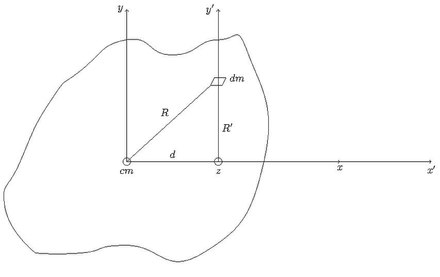
\includegraphics[width = 8cm]{huygen}	
\centering
\end{figure}
 \begin{proof}
 	Si consideri un sistema di riferimento cartesiano (x,y) con l'origine nel centro di massa e un altro sistema di riferimento tralsato lungo l'asse x di una certa quantit\`{a}, in modo tale che y = $\text{y}^{\prime}$  e $x = \text{x}^{\prime} -d$, dove d \`{e} la distanza tra l'asse passante per il centro di massa e quella parallelo di rotazione (rispetto al quale calcoliamo il momento).
 	\newline
 	
 	\noindent Si consideri un elemento infinitesimo \textit{dm}, il cui momento di inerzia rispetto al centro di massa \`{e} dato da $dI = R^2dm$. Integrando lungo tutto il corpo rispetto al centro di massa si ha che
 	\begin{equation*}
 		I_{cm} = \int_{S}(x^2 + y^2)dm
 	\end{equation*}
analogamente il centro di massa rispetto all'asse traslato \`{e} dato da 
\begin{equation*}
	I_{z} = \int_{S}(x'^{2}+y'^{2})dm  
\end{equation*}
applicando le trasformazione nel sistema rispetto al SR precedente si ha
\begin{equation*}
	I_{z} = \int_{S}[(x+d)^2+y^2]dm = \int_{S}[x^2+y^2]dm + d^2 \int_{S}dm   \;+ 2d \int_{S}xdm
\end{equation*}
l'ultimo termine \`{e} nullo in quanto l'integrale di xdm \`{e} l'ascissa del centro di massa nel SR del centro di massa stesso.
\begin{equation*}
	I_{z} = I_{cm} + Md^2
\end{equation*} 
 \end{proof}

\subsection{Tensore d'inerzia}

Nella sezione sulle velocit\`{a} angolari abbiamo visto che la velocit\`{a} di un punto in rotazione pu\`{o} essere scritta come 
\begin{equation}
	\bm{\dot{x}} = \Omega \bm{x} 
\end{equation}
dove $\Omega = R^T\dot{R}$ che \`{e} una matrice anti-simmetrica e in generale ha forma 
\begin{equation}
\Omega=\left[\begin{array}{ccc}
0 & -\Omega_3 & \Omega_2 \\
\Omega_3 & 0 & -\Omega_1 \\
-\Omega_2 & \Omega_1 & 0
\end{array}\right]
\end{equation}
dove ogni elemento della matrice \`{e} esprimibile come $\Omega_{ik} = - \varepsilon^{lik}\omega_{l}$ con l,i,k distinti tra loro. Il simbolo $\varepsilon^{lik}$ prende il nome di tensore di Levi-Civita.
Possiamo scrivere la matrice $\Omega$ rispetto un'opportuna base $\{ E_i\}$, nel seguente modo
\begin{equation}
	\Omega = \Omega_1 \bm{E}_1 + \Omega_2 \bm{E}_2 + \Omega_3 \bm{E}_3
\end{equation}
dimostriamo che la relazione 4.25 pu\`{o} essere riscritta come
\begin{equation}
	\dot{\bm{x}} = \Omega\bm{x} = \Omega \times \bm{x}
\end{equation}
la componente lungo $\bm{E}_{1}$ di $\bm{x}$ \`{e} data da 
\begin{equation}
	\bm{E}_1 \cdot \Omega \cdot \bm{\dot{x}} = det \left [ \begin{array}{ccc}
		\bm{E}_1 & \bm{E}_{2} & \bm{E}_{3} \\
		\Omega_{1} & \Omega_{2} & \Omega_{3}\\
		x_1 & x_1 & x_1
	\end{array}\right] \cdot \bm{E}_{1} = \Omega_{3}x_{2} + \Omega_{2}x_{3}
\end{equation}  
in modo analogo si definisco le altre componenti lungo $\bm{E}_2$ ed $\bm{E}_3$. Scriviamo l'energia cinetica del punto rispetto alla nuova notazione nel seguente modo
\begin{equation}
\begin{aligned}
	& K_{x} = \frac{1}{2}m ||\bm{\dot{x}}||^2 = \frac{1}{2}m ||\Omega \times \bm{x}||^2 = \frac{1}{2}m||\Omega||^2||\bm{x}||^2sin^2(\widehat{\Omega \bm{x}}) = &\\[0.2in]
	& =\frac{1}{2}m \left [ ||\Omega||^2||\bm{x}||^2 - ||\Omega||^2||\bm{x}||^2cos^2(\widehat{\Omega \bm{x}}) \right ] = &\\[0.2in]
	& = \frac{1}{2} \left [ ||\Omega||^2||\bm{x}||^2 - ( \Omega \cdot \bm{x})^2 \right ] = & \\[0.2in]
	& = \frac{1}{2}m \left [ \sum_{j} \Omega_j^2||\bm{x}||^2 + \sum_{j}\Omega_j y_j \sum_{k} \Omega_k y_k \right ] = (*)
\end{aligned}
\end{equation}
il primo termine pu\`{o} essere esplicitato come
\begin{equation}
	\sum_{j} \Omega_j^2 = \sum_{jk}\Omega_j \Omega_k \delta_{jk}
\end{equation}
dove $\delta_{jk}$ \`{e} il delta di Kroeneker. In questo modo la relazione 4.30 diventa
\begin{equation}
	=\frac{1}{2}m \left [ \sum_{jk} \Omega_j (||\bm{x}||^2 \delta_{jk} - y_j y_k)\Omega_k\right ]
\end{equation}
l'energia totale per un sistema di N particelle sar\`{a} data da 
\begin{equation}
	K = \frac{1}{2} \left \{\sum_{\alpha}^N m_{\alpha} \left [ \sum_{jk} \Omega_j (||\bm{x}_{\alpha}||^2 \delta_{jk} - y_j^{\alpha} y_k^{\alpha})\Omega_k\right ] \right \}  
\end{equation}
il termine 
\begin{equation}
	\left [ \sum_{jk} \Omega_j (||\bm{x}||^2 \delta_{jk} - y_j y_k)\Omega_k\right ] = I_{jk}
\end{equation}
\`{e} il momento d'inerzia $I_{jk}$ del \textbf{tensore d'inerizia} dove i termini $y_{\alpha}$ sono espressi rispetto SR del centro di massa. Per un corpo esteso la relazione 4.34 assume la forma 
\begin{equation}
	I_{jk} = \int_{V}dx_1\,dx_2\,dx_3\,\rho(x_1,x_2,x_3)\left [  \delta_{jk} ||\bm{x}||^2 - y_jy_k\right ]
\end{equation}
Il tensore d'inerzia \`{e} una matrice simmetrica della forma 
\begin{equation}
\hat{I} = 
\left[\begin{array}{ccc}
\int_V d V \rho\left[x_2^2+x_3^2\right] & -\int_V dV \rho\left(x_1 x_2\right) & -\int_V dV\rho \left(x_1 x_3\right) \\[0.2in]
\prime \prime & \int_V d V \rho\left[x_1^2+x_3^2\right] & -\int_V dV \rho\left(x_2 x_3\right) \\[0.2in]
\prime \prime & \prime \prime & \int_V dV \rho\left[x_1^2+x_2^2\right]
\end{array}\right]
\end{equation}
\begin{wrapfigure}[7]{l}{0.6\textwidth}
  \begin{center}
    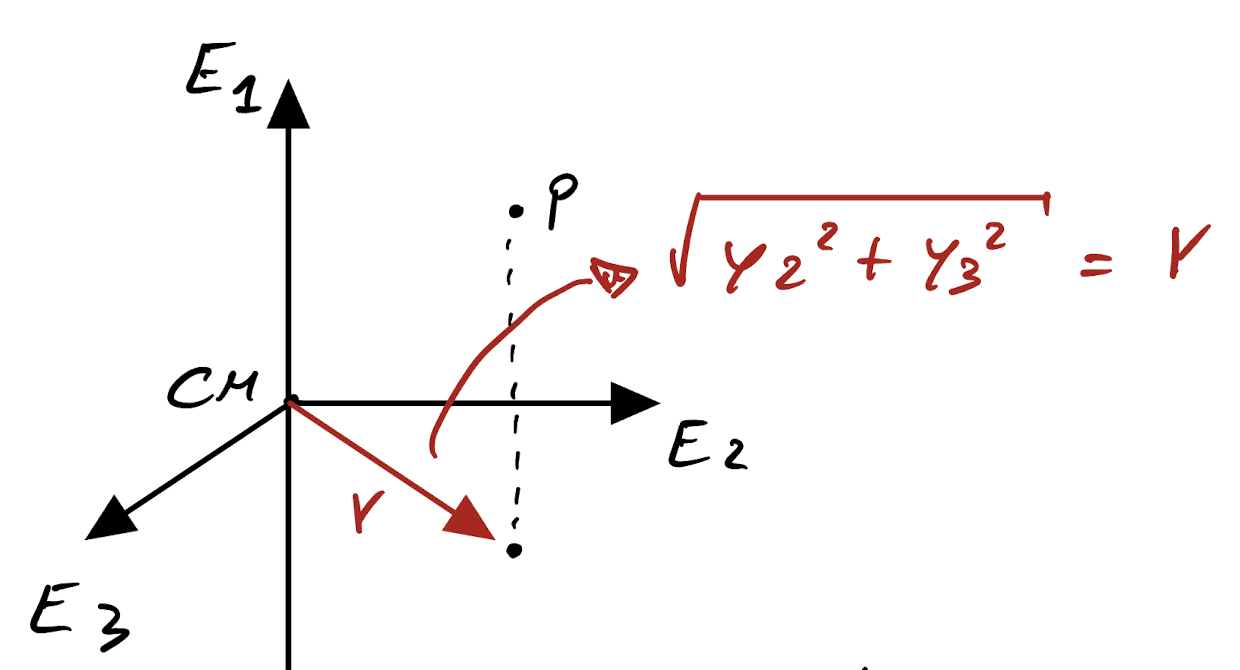
\includegraphics[width=0.6\textwidth]{inertia}
    \end{center}
\end{wrapfigure}

\vspace{0.3in}
\noindent Il primo termine del tensore \`{e} dato da $I_{11}$, avremo che \`{e} equivalente alla massa in un punto pesata rispetto il quadrato della distanza dall'asse di rotazione $\bm{E}_1$.\newline

\noindent Analogamente nelle altre direzioni.

\begin{remark}
	\noindent Notare che non sono state fatte ipotesi sull'orientazione degli assi $\bm{E}_{i}$ tantomeno che essi costituiscano una base ortonormale. Infatti nella forma generale del tensore d'inerzia compaiono altri termini oltre a quelli della diagonale. Essendo per\`{o} la matrice simmetrica questa risulta essere diagonalizzabile. 
\end{remark}

\noindent Si prendamo $\bm{E}_1^{\prime}, \bm{E}_2^{\prime}, \bm{E}_3^{\prime}$ in modo tale che la matrice d'inerzia sia diagonale, applicando una matrice $S \in SO(3)$ alla base di partenza in modo tale che $R^{\prime} = SR$. In questo modo la base $\bm{E}^{\prime}$ \`{e} aggiustata rispetto alle simmetrie del corpo rigido. Poich\`{e} S non dipende dal tempo la matrice $\Omega$ 
\begin{equation*}
	\Omega^{\prime} = R^{\prime^T} \dot{R}^{\prime} = R^TS^TS\dot{R} = R^T\dot{R} = \Omega
\end{equation*}
rimane invariata. In questo modo la matrice del tensore d'inerzia assume la forma 
\begin{equation}
\hat{I} =
\left[\begin{array}{ccc}
I_{11} & 0 & 0 \\
0 & I_{22} & 0 \\
0 & 0 & I_{33}
\end{array}\right]
\end{equation}
dove gli elementi lungo la diagonale prendono il nome di \textbf{momenti principali d'inerzia}.
\subsubsection{Esempio: La Sbarra}
Si consideri il tensore d'inerzia di una sbarra uniforme di lunghezza L e massa M rispetto al suo centro. La densit\`{a} della sbarra \`{e} da da $\rho = \frac{M}{L}$. Per simmetria avremo che $\hat{I} = diag(I_1,I_2,0)$ dove 
\begin{equation}
	I_1 = \int_{-\frac{L}{2}}^{\frac{L}{2}}\rho \, x^2 \,dx = \frac{1}{12}ML^2
\end{equation}
\subsubsection{Esempio: Lamina Rettangolare}
Consideriamo il tesnore d'inerzia di una lamina rettangolare di lato minore B e lato maggiore A e di massa M.La densit\`{a} della lamina \`{e} data da $\rho = \frac{M}{AB}$. Per simmetria si avr\`{a} la matrice di forma diagonale della forma
\begin{equation*}
\begin{aligned}
\hat{I} = 
	&\left [  \begin{array}{ccc}
  	\int_{S}\rho y^2dzdy & 0 & 0 \\[0.1in]
  	0 & \int_{S} \rho x^2 dxdz & 0 \\[0.1in]
  	0 & 0& \int_{S} \rho (x^2 + y^2)dxdy
  \end{array}
\right] =&\\[0.25in] = 
	&\left [  \begin{array}{ccc}
  	\frac{1}{12}Mb^2 & 0 & 0 \\[0.1in]
  	0 & \frac{1}{12}Ma^2 & 0 \\[0.1in]
  	0 & 0& \frac{1}{12}Mr^2
  \end{array}
\right]
\end{aligned}
\end{equation*}
\subsubsection{Esempio: Il Disco}
Prendiamo un disco uniforme di raggio r e massa M. Per simmetria abbiamo che $\hat{I} = diag(I_1,I_2,I_3)$. La densit\`{a} del disco \`{e} data da $\rho  = \frac{M}{\pi r^2}$. L'espressione dei momenti principali coincide con quella della lamina rettangolare e quindi la matrice del tensore d'inerzia \`{e} data da 
\begin{equation*}
	\hat{I} = 
	\left [  \begin{array}{ccc}
  	\frac{1}{4}Mr^2 & 0 & 0 \\[0.1in]
  	0 & \frac{1}{4}Mr^2 & 0 \\[0.1in]
  	0 & 0& \frac{1}{2}Mr^2
  \end{array}
\right]
\end{equation*}
\subsubsection{Esempio: Sistema di dischi}
Consideriamo un disco di densit\`{a} $\rho_1$ e raggio 2R con all'interno altri due dischi che toccano in un punto A tra loro e di desnit\`{a} $\rho_2$ e raggio R, per calcolare il momento d'inerzia del sistema usiando il teorema di Huygen-Steiner.
\begin{equation*}
\begin{aligned}
	& I = I_{z,cm}(\rho_1,2R) + 2I_{z,A}(\rho_2 ,R) = &\\[0.1in]
	& = \frac{M_1}{2}4R^4 +2 \left (\frac{M_2}{2}R^2 + M_2 R^2 \right)
\end{aligned}
\end{equation*}
12
\subsection{Energia cinetica generalizzata}
Recuperando la relazione 4.20 usata nella sezione sull'energia cinetica
\begin{equation*}
\frac{1}{2}M\left\|\bm{\dot{x}}_0\right\|^2+\frac{1}{2} \sum_{p=1}^N m_p\left\|\dot{\bm{x}}_p\right\|^2+\left\langle\bm{\dot{x}}_0, \sum_{p=1}^N m_p \dot{\bm{x}}_p\right\rangle
\end{equation*}
siamo giunti alla espressione 4.23 poich\`{e} la quantit\`{a} di moto era espressa rispetto al riferimento del centro di massa e dunque era nulla. In conseguenza abbiamo potuto scrivere l'energia cinetica del sistema come somma di due termini. In generale tale risultato non \`{e} sempre possibile averlo e di conseguenza l'energia cinetica non \`{e} sempre somma di due termini. Per ottenere l'equazione 4.23 \`{e} necessario che sia abbia almeno un punto fisso non necessariamente solidale con il corpo rigido, ma comovente.

\section{Momento Angolare}

Definiamo momento angolare di un punto materiale P, rispetto ad un polo O la grandezza 
\begin{equation}
	\bm{L}_{O} = \int \rho dV \left [ \overline{OP} \times \dot{\overline{OP}}\right] = \int \rho dV \left [ \bm{x} \times \dot{\bm{x}}\right ] 
\end{equation}
essendo il moto rigido, ovvero la distanza $\overline{OP}$ non dipende dal tempo possiamo definire $\bm{\dot{x}} = \Omega \times \bm{x}$, e dunque 4.40 pu\`{o} essere riscritto come
\begin{equation}
	\bm{L}_{O} = \int \rho dV \left [ \bm{x} \times (\Omega \times \bm{x} \right ] = (*)
\end{equation}
prima di riscrivere la 4.41 introduciamo un lemma utile a tale fine.
\begin{lemma}
	\begin{equation}
		\bm{x} \times (\bm{z} \times \bm{x}) = ||\bm{x}||^2 \bm{z} - \langle \bm{x},\bm{z}\rangle \cdot \bm{x}
	\end{equation}
\end{lemma}
\begin{proof}
	Abbiamo che $\bm{z} \times \bm{x}$ \`{e} ortogonale al piano (x,z) di conseguenza il termine $\bm{x} \times (\bm{z} \times \bm{x})$ \`{e} ortogonale ad $\bm{x}$ e quindi pu\`{o} essere scritto come 
	\begin{equation*}
	\bm{x} \times (\bm{z} \times \bm{x}) = \alpha \bm{x} + \beta \bm{z}	
	\end{equation*}
di conseguenza possiamo definire due termini 
\begin{equation*}
\begin{aligned}
& 1)\quad \bm{x} \cdot(\bm{x} \times (\bm{z} \times\bm{x}))  = \alpha\|\bm{x}\|^2+\beta(\bm{x} \cdot \bm{z})=0 \\[0.1in]
& 2)\quad \bm{z} \cdot(\bm{x} \times(\bm{z} \times\bm{x})) = \alpha(\bm{x} \cdot \bm{z})+\beta\|\bm{z}\|^2 = 0
\end{aligned}
\end{equation*}
dalla equazione 1) abbiamo un sistema 
\begin{equation*}
	\left \{ \begin{array}{l}
		\|\bm{z} \times \bm{x} \|^2 = \alpha \langle \bm{x},\bm{z}\rangle + \beta \|\bm{z}\|^2 \\[0.1in]
		\alpha \|\bm{x}\|^2 + \beta \langle \bm{x},\bm{z} \rangle = 0
	\end{array} \right.
\end{equation*}
poich\`{e} 
\begin{equation*}
\begin{aligned}
\|\bm{z} \times \bm{x}\|^2 & =\|\bm{x}\|^2\|\bm{z}\|^2 \sin ^2\left({\widehat{\bm{x}\bm{z}}}\right) = \\
& \left.=\|\bm{x}\|^2\|\bm{z}\|^2\left(1-\cos ^2(\widehat{\bm{x}\bm{z}})\right)=\|\bm{x}\|^2\|\bm{z}\|^2-\langle \bm{x}, \bm{z}\right\rangle^2
\end{aligned}
\end{equation*}
di conseguenza sostituendo nel sistema abbiamo determiniamo $\alpha $ e $\beta$ come
\begin{equation*}
	\alpha = - \langle \bm{x},\bm{z} \rangle \quad \quad \beta = \|\bm{x}\|^2
\end{equation*}
\end{proof}
\noindent Usando il lemma 4.3.1 terminiamo l'espressione del momento angolare in 4.41 
\begin{equation}
\begin{aligned}
	&(*) = \int \rho dV \left [ \|\bm{x}\|^2 \bm{\Omega} - \langle \bm{x}, \bm{\Omega} \rangle \bm{x} \right ] = & \\[0.1in] 
	&= \sum_{j=1}^{3} \bm{E}_{j} \int \rho dV \left [ \sum_{k} \|\bm{x}\|^2 \delta_{jk}\Omega_k - y_k\Omega_k y_j \right ] = \\[0.1in]
	& = \sum_{j=1}^{3} \bm{E}_{j} \int \rho dV \sum_{k} \left [ \|\bm{x}\|^2 \delta_{jk}\Omega_k - y_k y_j \right ]\Omega_k = & \\[0.1in]
	& = \sum_{j=1}^3 \sum_{k} I_{jk}\Omega_{k} 
	\end{aligned}
\end{equation}
in conclusione 
\begin{equation}
	\bm{L}_{O} = \hat{I}\cdot \bm{\Omega}
\end{equation}
per $\bm{\Omega} = \sum_{j} \Omega_j \bm{E}_{j}$. Si osserva che per un moto libero il momento angolare costituisce una costante del modo. 
\begin{remark}
Il tensore d'inerzia da un punto di vista energetico fornisce l'informazione sul contributo dell'energia cinetica data dal moto rigido interno. Dal punto di vista dell'analisi meccanica \`{e} l'applicazione lineare, che usata sulla velocit\`{a} angolare restituisce il momento angolare.	
\end{remark}

\section{Equazioni di Eulero Per Il Corpo Rigido Libero}
In generale il moto di un corpo \`{e} descritto da una rotazione e una traslazione. Il polo rispetto a cui ruota il corpo pu\`{o} essere dato da un qualsiasi punto fisso, ma \`{e} utile utilizzare il centro di massa. Consideriamo un SR del laboratorio O e un sistema mobile $O^{\prime}$ solidale con il corpo rigido.

\noindent Ipotizzando che il corpo sia libero, ovvero non \`{e} soggetto a forze esterne, il suo momento angolare  rispetto al centro di massa \`{e} conservato.
\begin{equation}
	\frac{d\bm{L}_{cm}}{dt} = 0 
\end{equation}
L'equazione 4.45 diventa 
\begin{equation}
	\frac{d}{dt} \left ( \sum_{i} l_i \bm{e}_i \right ) = \sum_{i} \left ( \dot{l}_{i}\bm{e}_i + l_i \bm{\dot{e}}_{i} \right ) = \sum_{i} \dot{l}_{i} \bm{e}_{i} =0 \Rightarrow \dot{l}_i = 0
\end{equation}
il movimento del corpo rigido attorno al suo centro di massa, non \`{e} specificato dal momento angolare di per s\`{e} , ma dalla velocit\`{a} angolare.Infatti se esprimiamo il momento angolare usando l'equazione 4.44 abbiamo che le sue componenti 
\begin{equation}
	\frac{d}{dt}l_i = \frac{d}{dt}\left ( \sum_{k} I_{ik} \Omega_k \right ) = \sum_{k} \dot{I}_{ik}\Omega_k +I_{ik}\dot{\Omega}_k = 0 
\end{equation}
dove $I_{ik}$ sono le componenti del tensore d'inerzia viste da riferimento fisso. Poich\`{e} l'equazione 4.47 corrisponde ad un sistema di tre equazioni e nove incognite, questo non ammette soluzione rispetto al SR del laboratorio. Per risolverlo dobbiamo passare al SR mobile.
Dove rispettivamente valgono le operazioni di trasformazione sui vettori per una matrice $R \in SO(3)$ e dunque 
\begin{equation}
	\bm{E}_j = \sum_{k} R_{kj}\bm{e}_k \quad \bm{e}_{k} = \sum_{l} R_{kl} \bm{E}_{l}
\end{equation}
e il momento angolare \`{e} rispetto ad $O^{\prime}$ \`{e} dato da 
\begin{equation}
	\frac{d \bm{L}}{dt} = \frac{d}{dt} \left (\sum_{j}L_{j}\bm{E}_{j}\right ) = \sum_{j} \dot{L}_{j} \bm{E}_{j} + L_{j}\dot{\bm{E}}_{j} = 0
\end{equation}
utilizzando la definizione o del vettore $\bm{E}_{j}$ in 4.48 abbiamo che 
\begin{equation}
\begin{aligned}
	& \bm{\dot{E}}_{j} = \sum_{k} \dot{R}_{kj} \bm{e}_{k} + R_{kj}\dot{\bm{e}}_j = \sum_{k} = \sum_{k}\dot{R}_{kj} \sum_{l} R_{kl}\bm{E}_{l}= & \\[0.1in]
	& = \sum_{l} \sum_{k} \left ( R^T_{lk} \dot{R}_{kj}\right )\bm{E}_{l}
\end{aligned}
\end{equation}
utilizzando il risultato a 4.50 l'equazione 4.49 assume la forma 
\begin{equation}
	\begin{aligned}
		& \frac{d \bm{L}}{dt} = \sum_{l} \dot{L}_{l}\bm{E}_{l} + \sum_{j}\sum_{l} L_{j} \left (R^T \dot{R} \right )_{lj} \bm{E}_{l} = & \\[0.1in]
		& = \sum_{l} \left ( \dot{L}_{j} + \sum_{j}\left (R^T \dot{R} \right )_{lj} \right ) \bm{E}_{j} = \sum_{l} \left ( \dot{L}_{l} + \left ( \bm{\Omega} \times \bm{L} \right )_{l} \right )\bm{E}_{l} = 0
	\end{aligned}
\end{equation}
in questo modo si ottiene un sistema di tre equazioni in tre incognite 
\begin{equation}
	\left \{ \begin{array}{l}
		\dot{L}_{1} + \left ( \bm{\Omega} \times \bm{L} \right )_{1} = 0 \\[0.1in]
		\dot{L}_{2} + \left ( \bm{\Omega} \times \bm{L} \right )_{2} = 0\\[0.1in]
		\dot{L}_{3} + \left ( \bm{\Omega} \times \bm{L} \right )_{3} = 0
	\end{array} \right.
\end{equation}
che ammette soluzione. Poich\`{e} il tensore d'inerzia \`{e} simmetrico e quindi risulta essere sempre diagonalizzabile possiamo considerare per semplicit\`{a} la sua forma diagonale e dunque
\begin{equation}
	L_{k} = I_k \Omega_k \quad \text{e} \quad \dot{L}_{k} = \dot{I}_{k} \Omega_{k}  + I_k \dot{\Omega}_k = I_k \dot{\Omega}_k
\end{equation}
il sistema di equazioni 4.52 dunque pu\`{o} essere riscritto come 
\begin{equation}
	\left \{ \begin{array}{l}
		\dot{\Omega}_{1} = \left ( \frac{I_1 - I_3}{I_1} \right ) \;\Omega_2 \Omega_3  \\[0.1in]
		\dot{\Omega}_{2} = \left ( \frac{I_3 - I_1}{I_2} \right ) \;\Omega_1 \Omega_3 \\[0.1in]
		\dot{\Omega}_{3} = \left ( \frac{I_1 - I_2}{I_3} \right ) \;\Omega_1 \Omega_2
	\end{array} \right.
\end{equation}
tali relazioni prendono il nome di \textbf{equazioni di Eulero}  e dipendono dalla geometria del corpo rigido.	
\subsection{Ellissoide di Poinsot}
L'ellissoide di Poinsot \`{e} un metodo geometrico che ci permette di visualizzare il moto di un corpo rigido libero, ipotizzando di avere quattro costanti, date dall'energia cinetica e le tre componenti del momento angolare espresse rispetto a sistema di riferimento del laboratorio.



\section{Angoli di Eulero}

Fino a questo punto siamo riusciti a formulare buona parte della dinamica di un corpo rigido usando le le velocit\`{a} angolari, e non abbiamo avuto la necessit\`{a} di parametrizzare lo spazio delle configurazioni C. Per proseguire nella trattazione del corpo rigido abbiamo proprio bisogno di introdurre tale metodo.

 
\begin{figure}[!ht]
\vspace{0.1in}
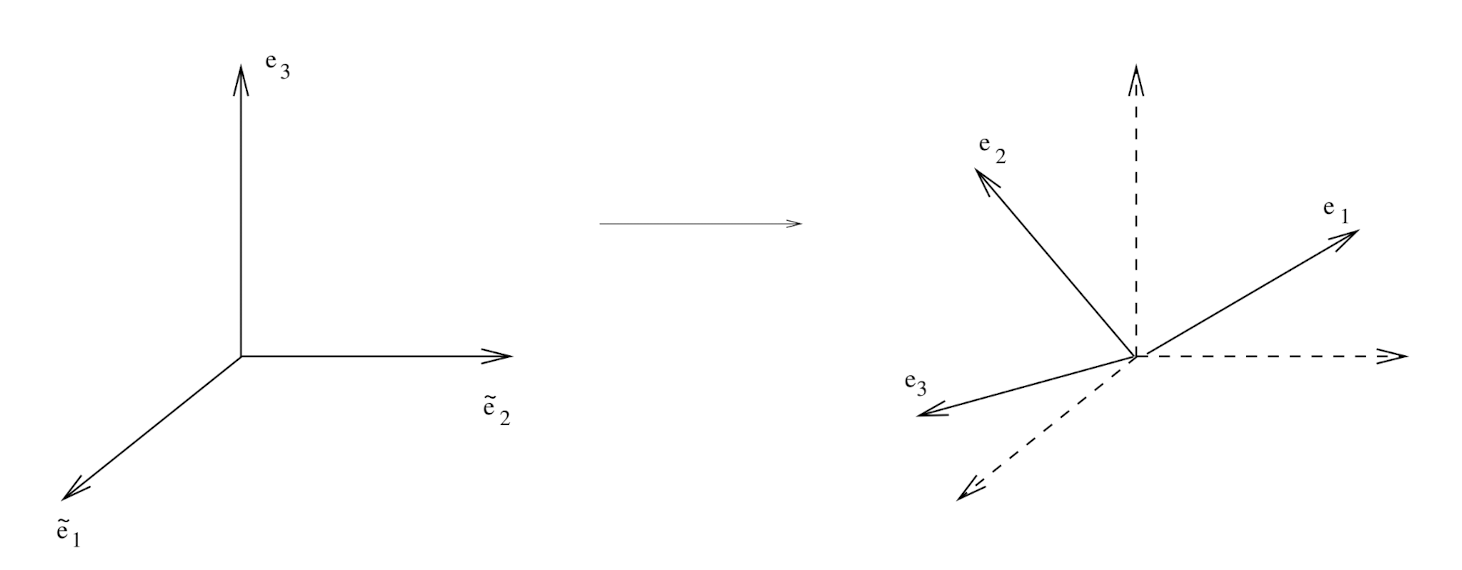
\includegraphics[width = 12cm]{rot}	
\centering
\vspace{0.1in}
\end{figure}

una rotazione generica di un insieme di assi \`{e} come quella mostrata in figura. L'obbiettivo \`{e} costruire un modo per parametrizzare tale rotazione. Un modo per farlo ci viene dato dagli studi di Eulero:

\begin{theorem}[\textbf{Teorema di Eulero}]
	Una rotazione arbitraria pu\`{o} essere espressa come il prodotto di 3 rotazioni successive rispetto ai 3 assi differenti.
\end{theorem}
\begin{proof}
	Sia $\{\tilde{\bm{e}}_{a}\}$ la base del sistema di riferimento fisso; e sia $\{\bm{e}_{a}\}$ la base del sistema mobile. Vogliamo determinare la rotazione R tale per cui $\bm{e}_{a} = R_{ab}\tilde{\bm{e}}_{b}$. Per ottenere tale risultato ci servono tre passi successivi
	\begin{equation*}
\left\{\tilde{\mathbf{e}}_a\right\} \xrightarrow{R_3(\phi)}\left\{\mathbf{e}_a^{\prime}\right\} \xrightarrow{R_1(\theta)}\left\{\mathbf{e}_a^{\prime \prime}\right\} \xrightarrow{R_3(\psi)}\left\{\mathbf{e}_a\right\}
\end{equation*}
Nel dettaglio abbiamo
\begin{itemize}
	\item \textbf{Passo 1:} Ruotare di un angolo $\phi$ l'asse $\bm{\tilde{e}}_3$. In questo modo $\bm{e}_{a}^{\prime} = R_3(\phi)\tilde{\bm{e}}_{b}$ con 
	\begin{equation*}
R_3(\phi)=\left(\begin{array}{ccc}
\cos \phi & \sin \phi & 0 \\
-\sin \phi & \cos \phi & 0 \\
0 & 0 & 1
\end{array}\right)
\end{equation*}
 
\begin{figure}[!ht]
\vspace{0.1in}
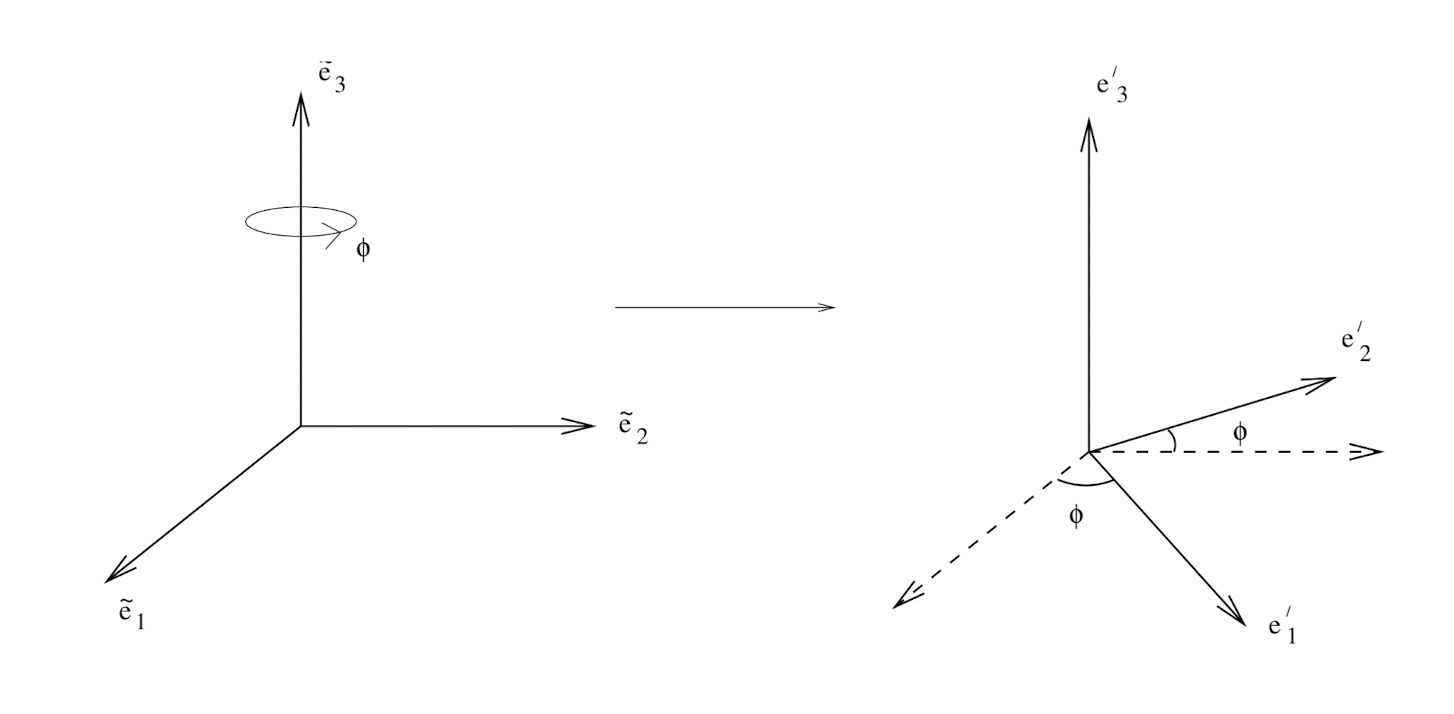
\includegraphics[width = 12cm]{e3}	
\centering
\vspace{0.1in}
\caption{Rotazione lungo l'asse $\bm{\tilde{e}}_3$ rispetto al SR fisso }
\end{figure}

\item \textbf{Passo 2:} Ruotare di un angolo $\theta$ rispetto all'asse $\bm{e}_{1}^{\prime}$. Definiamo $\bm{e}_{a}^{\prime \prime} = R_1(\theta)_{ab}\bm{e}^{\prime}_{b}$ rispetto alla matrice 
\begin{equation*}
R_1(\theta)=\left(\begin{array}{ccc}
1 & 0 & 0 \\
0 & \cos \theta & \sin \theta \\
0 & -\sin \theta & \cos \theta
\end{array}\right)
\end{equation*}

\begin{figure}[ht]
\vspace{0.1in}
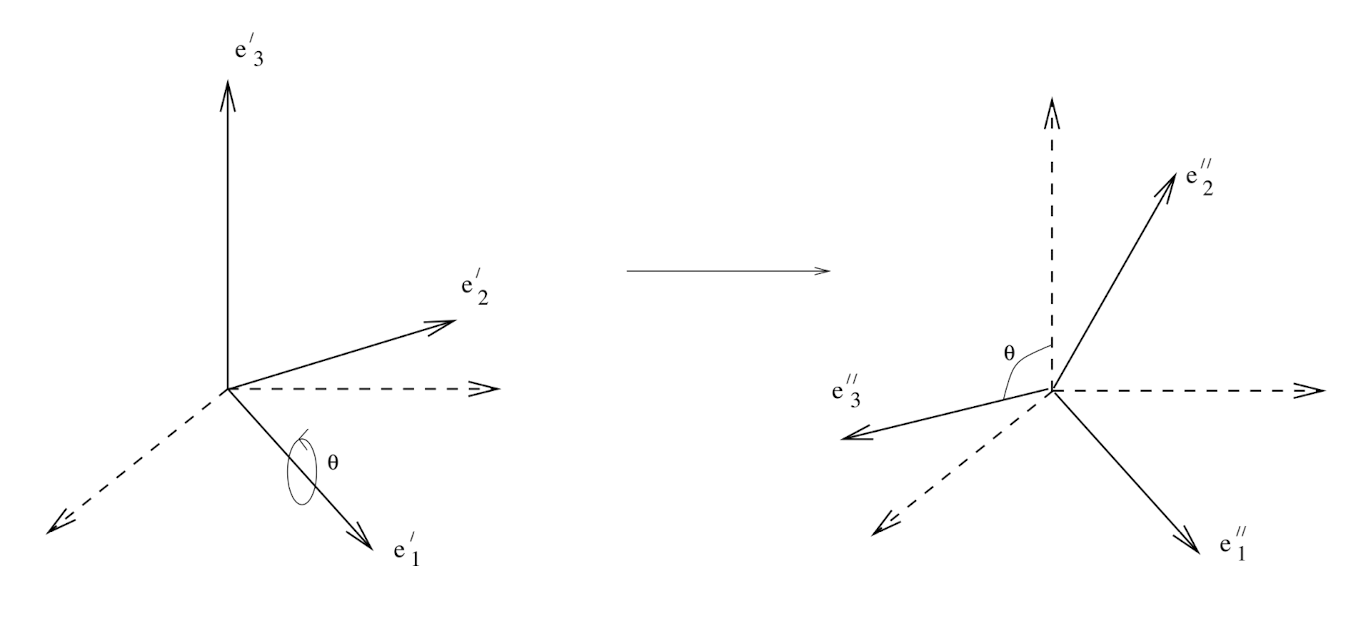
\includegraphics[width = 12cm]{e1}	
\centering
\vspace{0.1in}
\caption{Rotazione attorno all'asse $\bm{e}_{1}^{\prime}$}
\end{figure}

\item \textbf{Passo 3:} Ruotare di un angolo $\psi$ rispetto l'asse $\bm{e}_{3}^{\prime \prime}$ e quindi $\bm{e}_{a} = R_3(\psi)_{ab}\bm{e}_{b}^{\prime \prime}$ dove
\begin{equation*}
R_3(\psi)=\left(\begin{array}{ccc}
\cos \psi & \sin \psi & 0 \\
-\sin \psi & \cos \psi & 0 \\
0 & 0 & 1
\end{array}\right)
\end{equation*}

\begin{figure}[ht]
\vspace{0.1in}
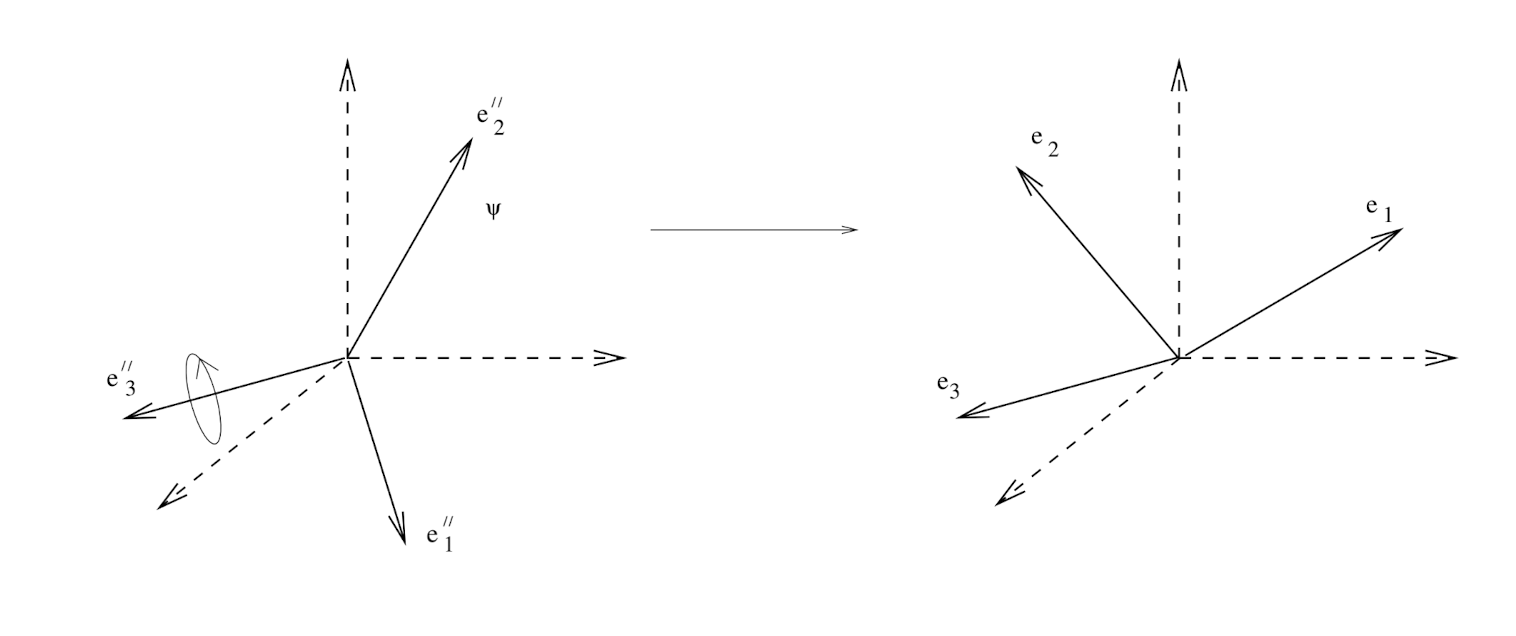
\includegraphics[width = 12cm]{ep3}	
\centering
\vspace{0.1in}
\caption{Rotazione attorno all'asse $\bm{e}_{3}^{\prime \prime }$}
\end{figure}

\end{itemize}
complessivamente abbiamo una composizione di applicazioni lineari della forma 
\begin{equation}
R_{a b}(\phi, \theta, \psi)=\left[R_3(\psi) R_1(\theta) R_3(\phi)\right]_{a b}
\end{equation}
\end{proof}
 
Gli angoli $\phi,\theta, \psi$ prendono il nome di \textbf{angoli d Eulero}. La matrice definita in 4.55 esplicitamente si scrive come 
\begin{equation*}
R=\left(\begin{array}{ccc}
\cos \psi \cos \phi-\cos \theta \sin \phi \sin \psi & \sin \phi \cos \psi+\cos \theta \sin \psi \cos \phi & \sin \theta \sin \psi \\
-\cos \phi \sin \psi-\cos \theta \cos \psi \sin \phi & -\sin \psi \sin \phi+\cos \theta \cos \psi \cos \phi & \sin \theta \cos \psi \\
\sin \theta \sin \phi & -\sin \theta \cos \phi & \cos \theta
\end{array}\right)
\end{equation*}
\newpage
\subsection{Velocit\`{a} Angolare}
Per ottenere l'espressione delle velocit\`{a} angolari istantanee in termini di angoli di Eulero \`{e} sufficiente sostituire l'espressione 4.55 all'interno dell'equazione 4.13. Siccome il procedimento \`{e} tedioso, \`{e} pi\`{u} rapida la sua deduzione partendo dal suo significato fisico. Consideriamo un corpo rigido che in un tempo infinitesimo dt compie una rotazione avremo che 
\begin{equation}
(\psi, \theta, \phi) \rightarrow(\psi+d \psi, \theta+d \theta, \phi+d \phi)
\end{equation}
Dalla definizione di angoli di Eulero, la velocit\`{a} angolare dovr\`{a} essere della forma 
\begin{equation}
\boldsymbol{\Omega}=\dot{\phi} \tilde{\mathbf{e}}_3+\dot{\theta} \mathbf{e}_1^{\prime}+\dot{\psi} \mathbf{e}_3
\end{equation}
possiamo esprimere i primi due vettori come combinazione lineare della base del SR del laboratorio, infatti
\begin{equation}
\begin{aligned}
& \tilde{\mathbf{e}}_3=\sin \theta \sin \psi \mathbf{e}_1+\sin \theta \cos \psi \mathbf{e}_2+\cos \theta \mathbf{e}_3 \\
& \mathbf{e}_1^{\prime}=\cos \psi \mathbf{e}_1-\sin \psi \mathbf{e}_2
\end{aligned}
\end{equation}
rispetto ai quali possiamo esprimere $\bm{\Omega}$ in termini di angoli di Eulero rispetto al SR fisso
\begin{equation*}
\boldsymbol{\Omega}=[\dot{\phi} \sin \theta \sin \psi+\dot{\theta} \cos \psi] \mathbf{e}_1+[\dot{\phi} \sin \theta \cos \psi-\dot{\theta} \sin \psi] \mathbf{e}_2+[\dot{\psi}+\dot{\phi} \cos \theta] \mathbf{e}_3
\end{equation*}
in modo analogo possiamo esprimere $\bm{\Omega}$ rispetto al SR mobile.
\section{Trottola di Lagrange}

\begin{wrapfigure}[7]{l}{0.5\textwidth}
\vspace{-1.4cm}
  \begin{center}
    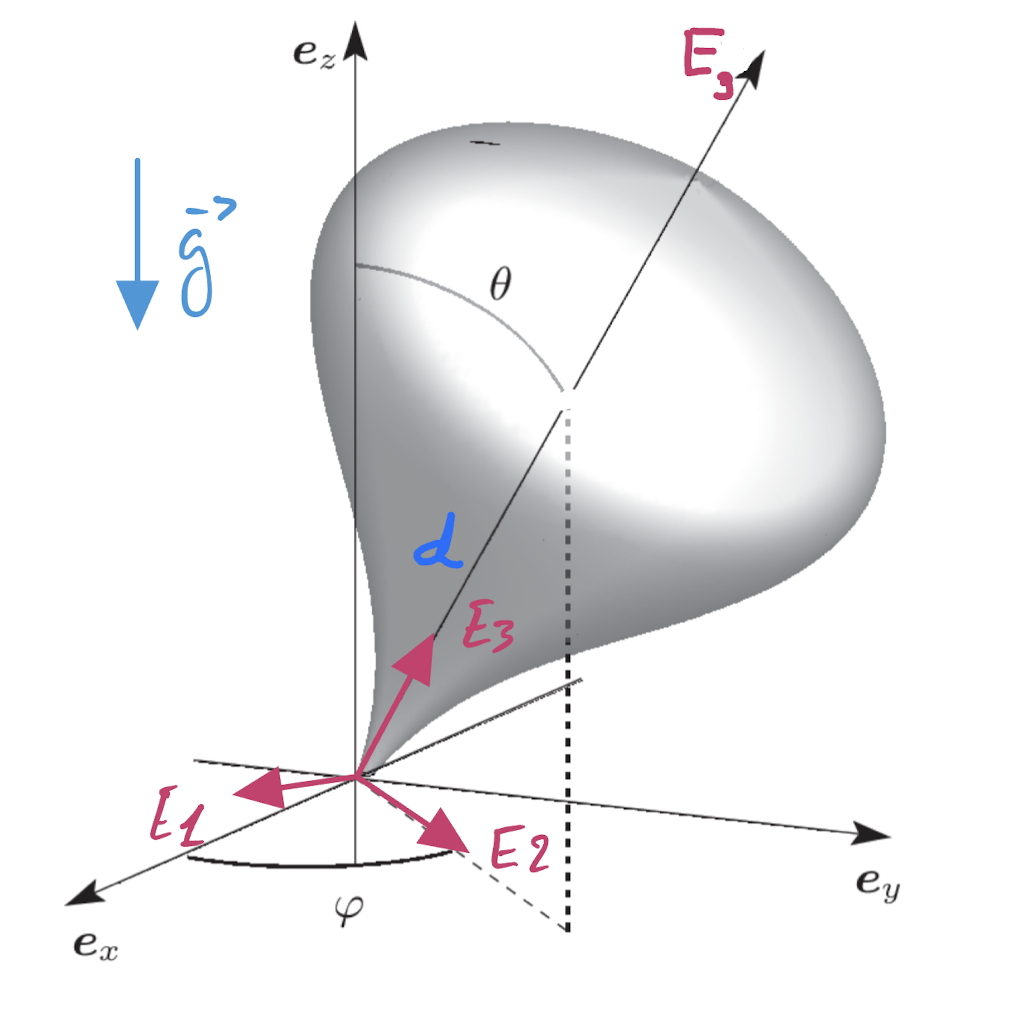
\includegraphics[width=0.4\textwidth]{trottola}
    \end{center}
\end{wrapfigure}

Consideriamo un corpo rigido simmetrico di massa M, fissato a ruotare rispetto ad un punto P, distante \textit{d} dal centro di massa. Gli assi principali del SR solidale sono $\{\bm{E}_i\}$. Inoltre su di esso agisce la forza di gravit\`{a}. 

\subsection{Studio dell'energia del sistema}
Dato che agisce solo la forza di gravit\`{a} e questa \`{e} una forza conservativa avremo che l'energia potenziale del sistema \`{e} data da 
\begin{equation}
	U(\theta) = \text{Mgz}_{cm} = \text{Mdcos}\theta
\end{equation}
mentre l'energia cinetica \`{e} esprimibile come 
\begin{equation}
	T = \frac{1}{2}\;\bm{\Omega}^{T}\hat{I}\;\bm{\Omega}
\end{equation}
essendo il corpo rigido simmetrico rispetto un'asse abbiamo che la matrice del tensore d'inerzia \`{e} diagonale $\hat{I} = diag(I_1,I_2,I_3)$. \newline
L'angolo $\varphi$ descrive la rotazione rispetto all'asse $\bm{e}_{3}$ del SR fisso, se cambiano l'origine, la descrizione fisica del problema rimane invariata di conseguenza \`{e} una coordinata che non d\`{a} nessun contributo all'equazione dell'energia cinetica. Analogo ragionamento per $\psi$. \newline
\begin{wrapfigure}{r}{0.5\textwidth}
\vspace{-1.4cm}
  \begin{center}
    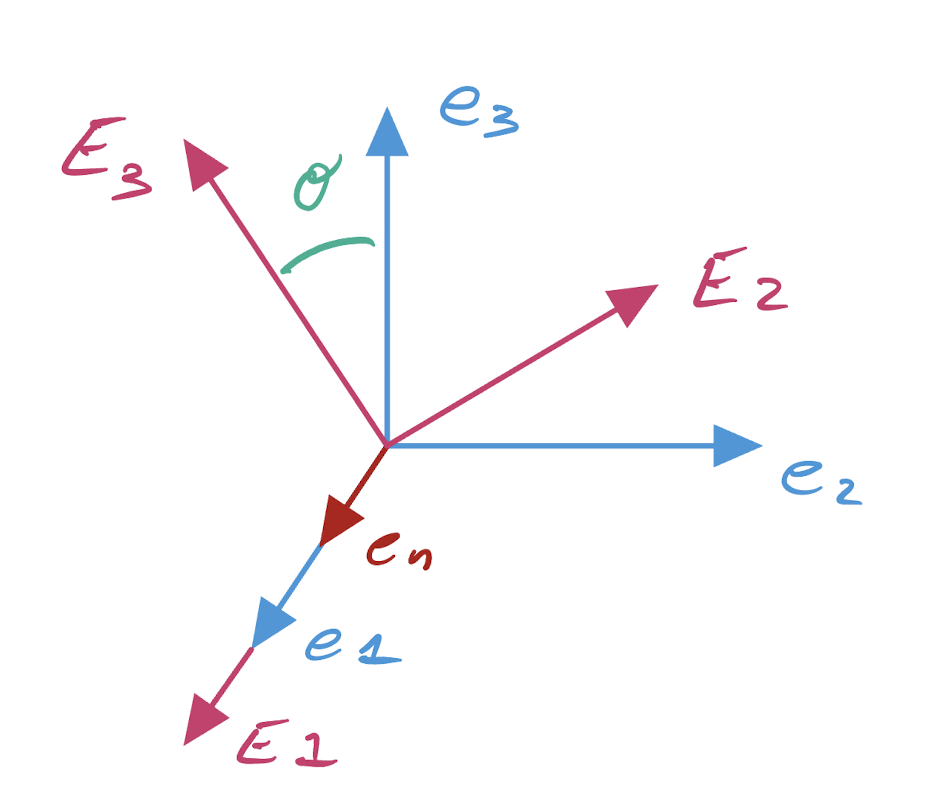
\includegraphics[width=0.5\textwidth]{piano}
    \end{center}
\end{wrapfigure}
Per calcolare l'energia cinetica possiamo ipotizzare che $\varphi$ e $\psi$ siano nulle e di conseguenza $\bm{e}_{3}$ giace nel piano formato dai vettore della base mobile $\{\bm{E}_2,\bm{E}_{3}\}$ e quindi esprimibile come 
\begin{equation}
	\bm{e}_{3} = \cos\theta \bm{E}_{3} + \sin \theta \bm{E}_{2}
\end{equation}
inoltrwe $\bm{e}_{1}^{\prime} = \bm{E}_{1}$ di conseguenza la velocit\`{a} angolare del sistema rispetto al SR mobile \`{e} data dalla seguente equazione 
\begin{equation}
\begin{aligned}
	& \bm{\Omega} = \dot{\varphi} \left ( \cos\theta \bm{E}_{3} + \sin \theta \bm{E}_{2} \right ) + \dot{\theta} \bm{E}_{1} + \dot{\psi}\bm{E}_{3} = & \\[0.15in]
	& = \dot{\theta} \bm{E}_{1} + \dot{\varphi}\sin \theta \bm{E}_{2} + \left ( \dot{\psi} + \dot{\varphi} \cos\theta\right )\bm{E}_{3}
\end{aligned}
\end{equation}
\newpage 
\noindent Per la simmetria del corpo il momento d'inerzia $I_{11} = I_{22}$ in conclusione la Lagrangiana del sistema \`{e} data da 
\begin{equation}
	\boxed{\mathcal{L} = \frac{1}{2} I_{11} \left ( \dot{\theta}^2 + \dot{\varphi}^2\sin^2\theta \right ) + \frac{1}{2}I_{33} \left ( \dot{\psi} + \dot{\varphi} \cos\theta \right )^2 - \text{Mgd}\cos \theta} 
\end{equation}

\begin{remark}
Se $I_{33} = 0$, cambiando i parametri si ottiene la Lagrangiana del pendolo sferico. 	
\end{remark}
\noindent Complessivamente abbiamo un problema a tre gradi di libert\`{a} con due costanti cicliche $\varphi$ e $\psi$. Che come sappiamo coincidono con la conservazione del momento angolare dei rispettivi assi.
\begin{equation}
	\left \{ \begin{array}{l}
		L_{z} = \frac{\partial \mathcal{L} }{\partial \dot{\varphi}} = I_{11}\dot{\varphi}\sin^2\theta + I_{33} \left ( \dot{\psi} + \dot{\varphi} \cos\theta \right )\cos \theta \\[0.2in]
		L_{3} = \frac{\partial \mathcal{L} }{\partial \dot{\psi}} = I_{33} \left ( \dot{\psi} + \dot{\varphi} \cos\theta \right )
	\end{array} \right.
\end{equation}
dove $L_{z}$ \`{e} rispetto l'asse $\bm{e}_{3}$ mentre $L_{3}$ rispetto ad $\bm{E}_{3}$.
Le equazioni E-L associate sono date da
\begin{equation}
	\left \{ \begin{array}{l}
		I_{11}\ddot{\theta} = I_{11} \sin \theta \cos \theta \dot{\varphi}^2 + I_{33} \left ( \dot{\psi} + \dot{\varphi} \cos\theta \right ) \sin \theta + Mgd \sin \theta \\[0.2in]
		\frac{d}{dt}L_{z} = \frac{d}{dt}L_{3} = 0
	\end{array} \right.
\end{equation}
mentre dalle grandezze conservate otteniamo le relazioni 
\begin{equation}
	\dot{\psi} = \frac{L_{z} - L_{3}\cos \theta}{I_{11} \sin^2 \theta } \quad \quad \dot{\varphi} = \frac{L_{3}}{I_{33}} - \frac{\cos \theta \left ( L_{z} - L_{3} \cos \theta \right)}{I_{11} \sin^2 \theta }
\end{equation}
a questo punto avendo due variabili cicliche possiamo definire la Lagrangiana ridotta, per farlo sostituiamo le relazioni in 4.66 all'interno dell'energia del sistema. 
\begin{equation}
	E_{eff} = \frac{1}{2} \dot{\theta}^2 + U_{eff}(\theta)
\end{equation}
dove 
\begin{equation}
	U_{eff}(\theta) = \frac{1}{2}\frac{ \left ( L_{z} - L_{3}\cos \theta \right )^2}{I_{11} \sin^2 \theta } + \text{Mgd}\cos\theta
\end{equation}
Da tale procedura si ottiene la Lagrangiana 
\begin{equation}
	\boxed{\mathcal{L}_{eff} = \frac{1}{2}I_{11} \dot{\theta}^2 - \frac{1}{2}\frac{ \left ( L_{z} - L_{3}\cos \theta \right )^2}{I_{11} \sin^2 \theta } - \text{Mgd}\cos\theta} 
\end{equation}
e rispettivamente le equazioni del moto sono date da 
\begin{equation}
	I_{11}\ddot{\theta} = - \frac{d U_{eff}(\theta)}{d\theta}
\end{equation}
che possono essere ottenute direttamente sostituendo le equazioni in 4.66 nel sistema 4.65. \newline
Il problema \`{e} stato ridotto allo studio di una sola variabile $\theta$ che costituisce la colatitudine del centro di rotazione, ovvero dell'asse passante per il centro di massa. Il moto avviene per valori fissati dell'energia dati dalle condizioni iniziali di velocit\`{a} e posizione.

\subsection{Studio qualitativo del moto}
Per studiare il moto introduciamo una variabile di supporto 
\begin{equation*}
	u = \cos \theta \quad \text{e} \quad \dot{u} =- \sin \theta \dot{\theta} \iff \dot{\theta} = - \frac{\dot{u}}{sin \theta}\quad \text{con} 
   \quad u \in [-1,1] 
\end{equation*}
per riscrivere le equazioni in modo conciso introduciamo anche due costanti 
\begin{equation}
\alpha=\frac{2 E_{eff}}{I_{11}} \quad \text { e} \quad \beta=\frac{2 M g d}{I_{11}}
\end{equation}
in questo modo le equazioni del moto 4.65 e le quantit\`{a} conservate 4.66 diventano 
\begin{equation}
\dot{u}^2=\left(1-u^2\right)(\alpha-\beta u)-(b-a u)^2 \equiv f(u)
\end{equation}
\begin{equation}
\dot{\phi}=\frac{b-a u}{1-u^2}
\end{equation}
\begin{equation}
\dot{\psi}=\frac{I_1 a}{I_3}-\frac{u(b-a u)}{1-u^2}
\end{equation}
Notiamo che la funzione f(u) definita in 4.72 \`{e} un polinomio cubico, e studiandone il comportamento otteniamo il grafico nella seguente figura.
 \newpage
\begin{figure}[!ht]
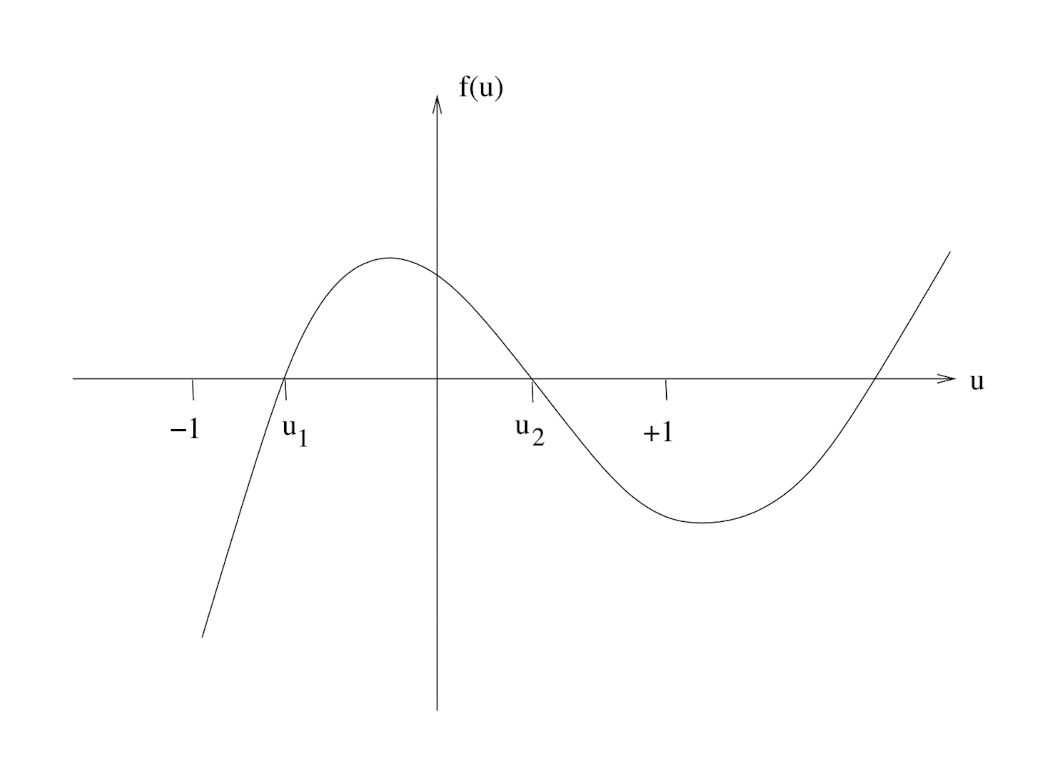
\includegraphics[width = 8cm]{cubic}	
\centering
\end{figure}
\noindent Poich\`{e} $f(u) \equiv \dot{u}^2 \geq 0 $ e $u \in [-1,1]$, si ha che il moto del sistema \`{e} confinato tra le due radici della funzione f(u). Se f(u) non interseca l'asse delle ascisse tale configurazione non \`{e} fisicamente realizzabile, per tali punti $\dot{u} = 0$ e quindi $\theta $ \`{e} una costante del moto. Le configurazioni del moto possibili sono:
\begin{itemize}

\item Se $f(u) \geq 0$ e si ha intersezione con l'asse delle ascisse si hanno le due radici $u_1$ e $u_2$, per i punti $u \in [u_1,u_2]$ si ha che il moto in $\theta$ \`{e} periodico in quanto confinato tra $\theta_{min}$ e $\theta_{max}$. L'asse $\bm{E}_{3}$ si muove tra i due estremi. Tale configurazione prende il nome di \textbf{moto di nutazione}. Inoltre $\dot{\varphi}$ cambia segno e la trottola cambia momentaneamente il moto.
\item Se $\bar{u} \notin [u_{1},u_{2}]$, $\dot{\varphi}$ ha segno costante e si ha sia una nutazione che una precessione nello stesso verso . 
\item Il caso limite \`{e} quando $\bar{u}$ \`{e} al limite dell'area consentita dove $\dot{\varphi} = 0$ in $u = u_2$ e $\dot{\varphi} > 0 $ in $u = u_1$. 
\end{itemize}
I moti rispetto $\varphi$ vengono definiti \textbf{moti di precessione}.
\begin{figure}[!ht]
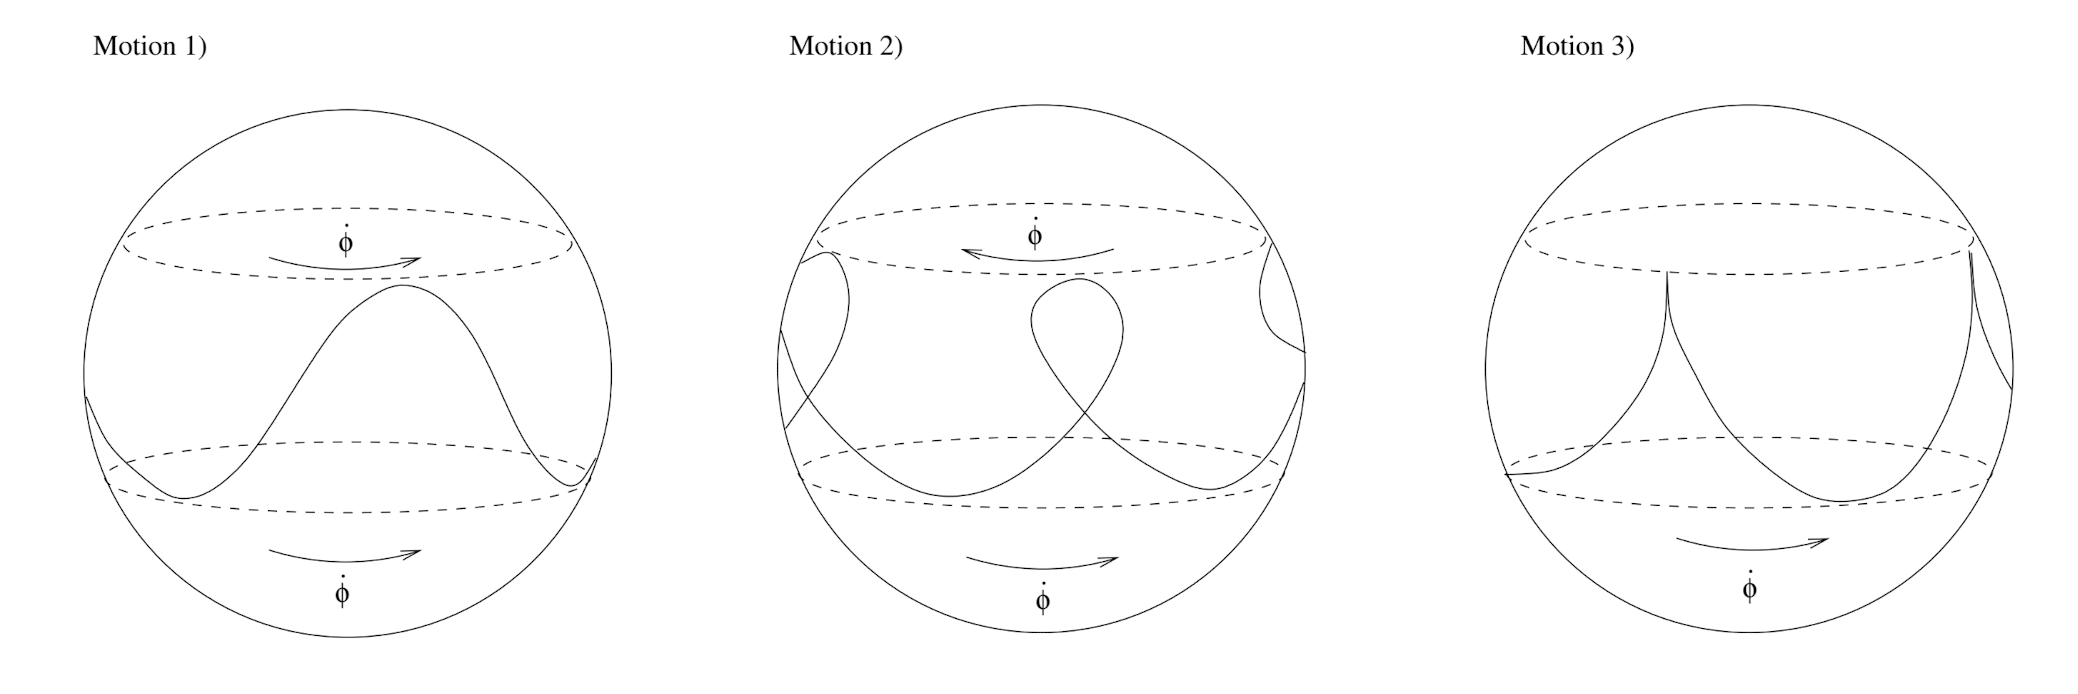
\includegraphics[width = 12.5cm]{motion}	
\centering
\end{figure}
